\documentclass[11pt]{article}
\pagestyle{headings}

\usepackage{fullpage}
\usepackage{graphicx}
\usepackage{sidecap}
\usepackage{subfig}
\usepackage{float}


\title{Tweet District Design Document}
\author{Victor Frolov}
\graphicspath{ {images/} }


\begin{document}
\maketitle

\section{Introduction}
Tweet District is an app that lets you find and interact with hundreds of tweets in your area (or any location of your choosing), and provides a way to find out about parties, local events, sales, promotions, and job hirings, and it's all shown on a map. Although it is currently a web app, it's use would be far greater on a mobile device. The purpose of this paper is to come up with a dream interface for this app, and use it as a guide during future development. Interaction design principles and theories are imperative to its development, and will range from usability measures, mental models, and many others.


\section{Landing Page}
Once a user downloads and opens the app, they will be greeted with a landing page with the logo, and app name that takes up a third of the screen. There will be one large button that allows the user to login to their existing twitter account (which will allow them to interact with the tweets, such as retweeting, sending direct messages, etc). Below the button will simply be clickable text that says "Use as Guest", allowing users to use the app without a twitter account. The logo, app name, button and text will be over a background color that will stay true to the app's theme. The background color will have opacity, and behind it there will be animations of users tweeting, partying, and shopping. 

% add an image to show what this looks like.


% talk about the navbar thingy on the bottom

\section{Main Page}
The main page is where all the magic happens. When I tried using the app on my mobile device when I was out and about with some friends, we found that there were a few issues impeding us from having a great experience. The first issue was having to type in a search word, check the current location box, and clicking search each and every single time we tried looking up something around us. See Figure 1.

\begin{figure}[H]
    \centering
    \subfloat[Current Search Appearance]{{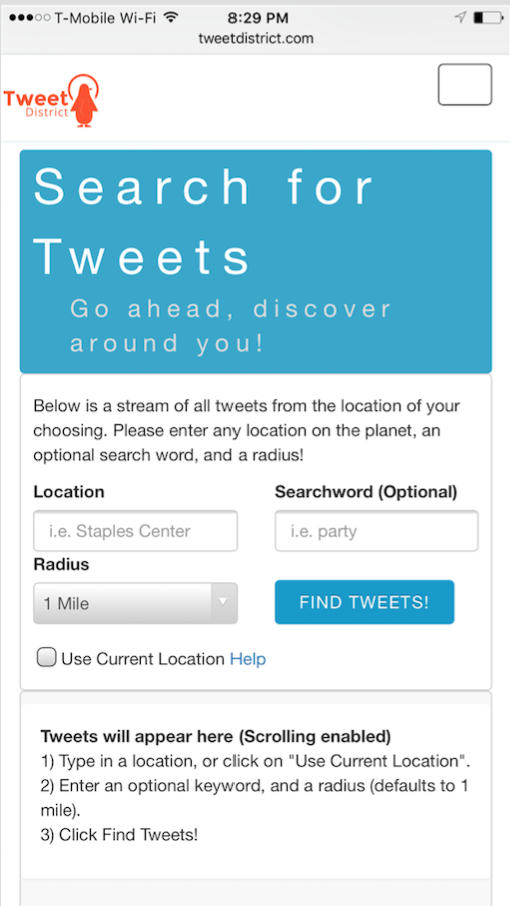
\includegraphics[width=7cm]{currentSearch} }}
    \qquad
    \subfloat[Simplified Search Appearance]{{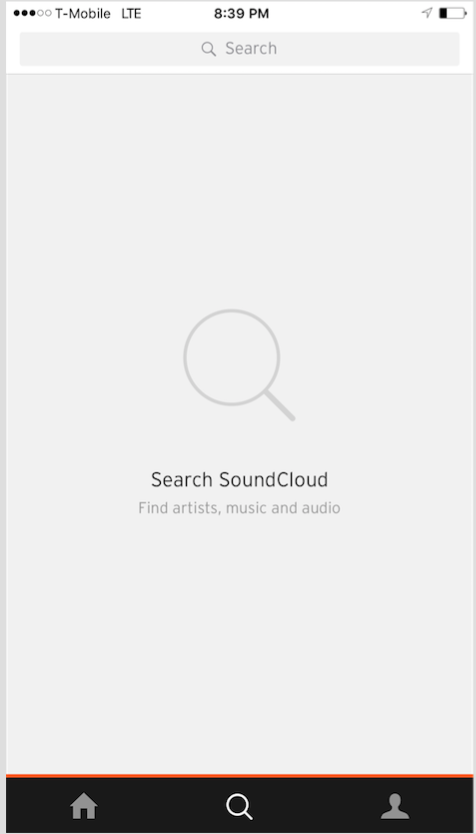
\includegraphics[width=7cm]{newSearch} }}
    \caption{Old Search and New Search Template}
    \label{fig:example}
\end{figure}

In order to overcome the first hurdle of having two repetitively check the box, put in a radius, search word, and click search for each search (we tried looking up about 10 keywords to find events around us, and although it ultimately worked, the process was arduous), a streamlined, preset 

Another was that, since the map takes almost the full screen, scrolling to and away from it it was difficult, as if the user tries to scroll down the page but is within the map box boundary, he would zoom in or out of the map. There was about a quarter inch of space both to the left and right of the map that allowed the user to scroll the page. 


%map scrolling image

Thirdly frustration was how to navigate between the map that had markers for all the tweets, and the box that displayed all the tweets in list form. Navigating between these two did not feel intuitive, and it felt like a burden.




% when talking about the main page, mention how when you were out it has to be easily accessible and searchable without any touch issues of scrolling (ie the map issue you currently have that takes up the full screen)


\end{document}
